%Thus far in this work a solution to simplify and automate design the process of all digital PLL loop filter designs comprised of (1) an automated loop filter optimization and design engine, and (2) a discrete-event, time domain PLL simulator to evaluate the designed filters with full time-discretization and quantization nonlinearity effects. I
In this discussion, the performance of the presented design solution will first be evaluated with a design example. Then, a comparison of the presented solution will be made to existing solutions in literature, pointing out advantages and disadvantages of this work. Finally, a general discussion will be made covering areas of improvement, reasoning for the central design choices made, and considerations for usage the framework.

\subsection{Design Exercise Using This Work}
The design of a loop filter for the PLL with the system level specifications of table \ref{design_specs} will be considered here, with the intent of optimizing total phase noise power (notated in this discussion as residual phase modulation). These specifications, where the TDC resolution in steps equals the divider ratio, is equivalent to a special case of a TDC-less PLL where a 150-step synchronous counter is used as a divider, and the loop filter directly samples the state of the synchronous counter. For the loop filter design, a PI-controller loop filter prototype was utilized in the optimizer due to its predictable phase margin and stability characteristics. Results of two design approaches with this framework will be presented. Approach 1 minimizes the residual phase modulation based on the TDC-phase detector PLL model. The BBPD gain in this case is optimized to minimize phase noise spectrum error in steady state for that expected from the TDC-PLL model. Approach 2 demonstrates loop filter optimization for both fast locking and low phase noise using loop filter gear switching. The first gear loop filter is optimized for minimum lock time using TDC feedback, and the second gear is optimized to minimize residual phase modulation in steady state using BBPD feedback.

% \scriptsize
\begin{table}[h!]
	\centering
	\def\arraystretch{1.5}		
	\setlength\arrayrulewidth{0.75pt}
	\setlength{\tabcolsep}{1em} % for the horizontal padding
	\begin{tabular}{|l|r|l|}
		\hline 
		\rule[-1ex]{0pt}{2.5ex} \cellcolor{gray!40}\textbf{Parameter} & \cellcolor{gray!40}\textbf{Value} & \cellcolor{gray!40}\textbf{Unit }\\ 
		\hline 
		\rule[-1ex]{0pt}{2.5ex} \textbf{Output Frequency}  & 2.4 & GHz \\ 
		\hline 
		\rule[-1ex]{0pt}{2.5ex} \textbf{Ref. frequency} & 16 & MHz\\ 
		\hline 
		\rule[-1ex]{0pt}{2.5ex} \textbf{Divider ratio} & 150  &\\ 
		\hline 
		\rule[-1ex]{0pt}{2.5ex} \textbf{TDC resolution} & 150  & steps/reference cycle\\ 
		\hline 
		\rule[-1ex]{0pt}{2.5ex} \textbf{DCO gain $K_{DCO}$} & $10^4$ & Hz/LSB \\ 
		\hline 
		\rule[-1ex]{0pt}{2.5ex} \textbf{DCO Phase noise} & -80 & dBc/Hz at $\Delta f=10^6$ Hz \\ 
		\hline 
		\rule[-1ex]{0pt}{2.5ex} \textbf{Lock Time} & $\leq$ 25 & $\mu$s \\ 
		\hline 
		\rule[-1ex]{0pt}{2.5ex} \textbf{Lock $\Delta f$ tolerance} & $10^5$ & Hz \\ 
		\hline 
		\rule[-1ex]{0pt}{2.5ex} \textbf{Digital filter word resolution} & $\leq$ 16 & bits \\ 
		\hline 
		\rule[-1ex]{0pt}{2.5ex} \textbf{Residual phase modulation} & minimize &  \\ 
		\hline 
	\end{tabular} 
	% \caption{Assigned specifications for branch line hybrid design.}
	% \label{asgn_specs}
	\caption{System-level specifications}
	\label{design_specs}
\end{table}   

\subsubsection{Approach 1: Results of Filter Optimization.}
Table \ref{filter_params} contains the optimized filter parameters obtained from the filter design optimizer developed in this work using the TDC based PLL model. $\{K$, $K_i$, $K_p$, $f_z\}$ are the continuous model parameters of section \ref{cont_pi_filt_des}, and $\{a_0$, $a_1$, $a_2$, $b_0$, $b_1\}$ are the filter coefficients for the discrete-time direct form-I filter structure of section \ref{disc_lf_comp_pi}. The estimated bandwidth for the filter is 144.8 kHz, and the lock time is estimated to be 19.3 $\mu$s. Table \ref{dig_filter_params} contains the digitized version of the discrete time filter, based on a selection for word size determined via optimization for finite word effects. The final data words are 13 bits in length.  
% \scriptsize
\begin{table}[h!]
	\centering
	\def\arraystretch{1.5}		
	\setlength\arrayrulewidth{0.75pt}
	\setlength{\tabcolsep}{1em} % for the horizontal padding
	\begin{tabular}{|l|r|l|}
		\hline 
		\rule[-1ex]{0pt}{2.5ex} \cellcolor{gray!40}\textbf{Parameter} & \cellcolor{gray!40}\textbf{Value} & \cellcolor{gray!40}\textbf{Unit }\\ 
		\hline 
		\rule[-1ex]{0pt}{2.5ex} \textbf{$K$}  & $1.343792\times10^{11}$ &  \\ 
		\hline 
		\rule[-1ex]{0pt}{2.5ex} \textbf{$K_i$}  & $1.343792\times10^{7}$ &  \\ 
		\hline 
		\rule[-1ex]{0pt}{2.5ex} \textbf{$K_p$}  & $7.331074\times10^{1}$ &  \\ 
		\hline 
		\rule[-1ex]{0pt}{2.5ex} \textbf{$f_z$} & $2.917324\times10^4$ & Hz\\ 
		\hline 
		\rule[-1ex]{0pt}{2.5ex} \textbf{$b_0$}  & $7.4150613906\times10^1$  &\\ 
		\hline 
		\rule[-1ex]{0pt}{2.5ex} \textbf{$b_1$}  & $-7.3310743796\times10^1$  & \\ 
		\hline 
		\rule[-1ex]{0pt}{2.5ex} \textbf{$a_0$}  & $1.0\times10^0$  &\\ 
		\hline 
		\rule[-1ex]{0pt}{2.5ex} \textbf{$a_1$}  & $-1.0\times10^0$  & \\ 
		\hline 
		\rule[-1ex]{0pt}{2.5ex} \textbf{$a_2$}  & $0.0\times10^0$  & \\ 
		\hline 
		\rule[-1ex]{0pt}{2.5ex} \textbf{$K_{bb}$}  & $3.007953\times10^{-2}$  & \\ 
		\hline 
		\rule[-1ex]{0pt}{2.5ex} Estimated bandwidth & $1.448234\times10^5$ & Hz \\ 
		\hline 
		\rule[-1ex]{0pt}{2.5ex} Estimated lock time & $1.934253\times10^{-5}$ & seconds \\ 
		\hline 
	\end{tabular} 
	% \caption{Assigned specifications for branch line hybrid design.}
	% \label{asgn_specs}
	\caption{PLL parameters determined from filter design and optimization process.}
	\label{filter_params}
\end{table}   

\begin{table}[h!]
	\centering
	\def\arraystretch{1.5}		
	\setlength\arrayrulewidth{0.75pt}
	\setlength{\tabcolsep}{1em} % for the horizontal padding
	\begin{tabular}{|l|r|r|l|}
		\hline 
		\rule[-1ex]{0pt}{2.5ex} \cellcolor{gray!40}\textbf{Parameter} & \cellcolor{gray!40}\textbf{Value} & \cellcolor{gray!40}\textbf{Value (digital) } & \cellcolor{gray!40}\textbf{Value Error}\\ 
		\hline 
		\rule[-1ex]{0pt}{2.5ex} Total dataword bits  & 13 & & \\ 
		\hline 
		\rule[-1ex]{0pt}{2.5ex} Sign bits  & 1 & & \\ 
		\hline 
		\rule[-1ex]{0pt}{2.5ex} Integer bits & 7 & & \\ 
		\hline 
		\rule[-1ex]{0pt}{2.5ex} Fractional bits  & 5 & & \\ 
		\hline 
		\rule[-1ex]{0pt}{2.5ex} \textbf{$b_0$} & $7.415625\times10^1$ & \texttt{0b0100101000101}  & $+5.636094\times10^{-3}$\\ 
		\hline 
		\rule[-1ex]{0pt}{2.5ex} \textbf{$b_1$}  & $-7.331250\times10^1$ & \texttt{0b1111011010110}  & $-1.756204\times10^{-3}$\\ 
		\hline 
		\rule[-1ex]{0pt}{2.5ex} \textbf{$a_0$}  & $1.0\times10^0$ & \texttt{0b0000000100000} & $0.0\times10^0$ \\ 
		\hline 
		\rule[-1ex]{0pt}{2.5ex} \textbf{$a_1$}  & $-1.0\times10^0$ & \texttt{0b1111111100000} & $0.0\times10^0$ \\ 
		\hline 
		\rule[-1ex]{0pt}{2.5ex} \textbf{$a_2$}  & $0.0\times10^0$ & \texttt{0b0000000000000} & $0.0\times10^0$ \\ 
		\hline 
		\rule[-1ex]{0pt}{2.5ex} \textbf{$K_{bb}$}  & $3.125\times10^{-2}$ & \texttt{0b0000000000001} & $+1.170461\times10^-3$ \\ 
		\hline 
	\end{tabular} 
	% \caption{Assigned specifications for branch line hybrid design.}
	% \label{asgn_specs}
	\caption{Loop filter parameters after digitization and optimization for data word length.}
	\label{dig_filter_params}
\end{table}  
\pagebreak

\subsubsection{Approach 1: Results of Transient and Phase Noise Simulation.}
The simulation engine implemented in this work was utilized to run a time domain simulation to verify the designed filter. Figures \ref{fig:trans_lf} and \ref{fig:trans_inst_freq} demonstrate the transient response of the PLL with an initial frequency error of 12 MHz (0.5\% of final frequency). It is observed that the PLL design stably approaches the target frequency in approximately 23 $\mu$s. Figures \ref{fig:trans_det} illustrate the BBPD and TDC outputs during this initial transient. It is observed that the TDC output gives the dominant feedback, until it reaches an output word of 0, where the BBPD then begins providing feedback in the steady state condition of the PLL. Figure \ref{fig:trans_phase_noise} is the result of a phase noise calculation for the simulated PLL in an interval beginning immediately after detection of lock. The spectrum closely approximates that designed for, with some small additional peaking.
	\begin{figure}[htb!]
	    \centering
	    \begin{subfigure}{0.5\textwidth}
	        \centering
	        \center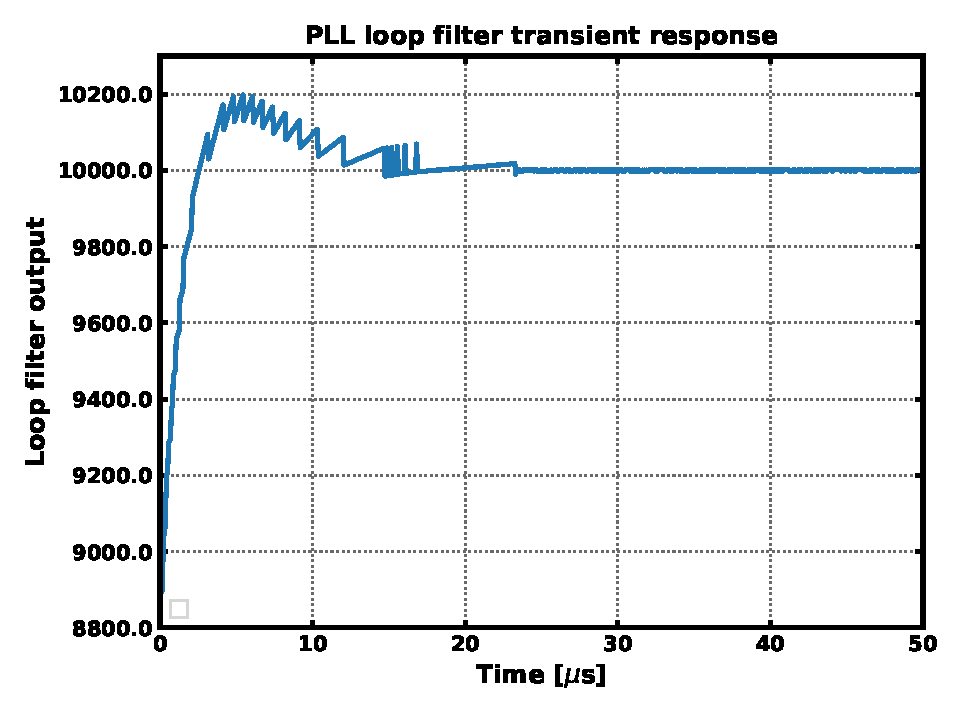
\includegraphics[width=1.0\textwidth, angle=0]{figs/trans_loop_filter.pdf}
	        \caption{ }
	        \label{fig:trans_lf}
	    \end{subfigure}%
	    \begin{subfigure}{0.5\textwidth}
	        \centering
	        \center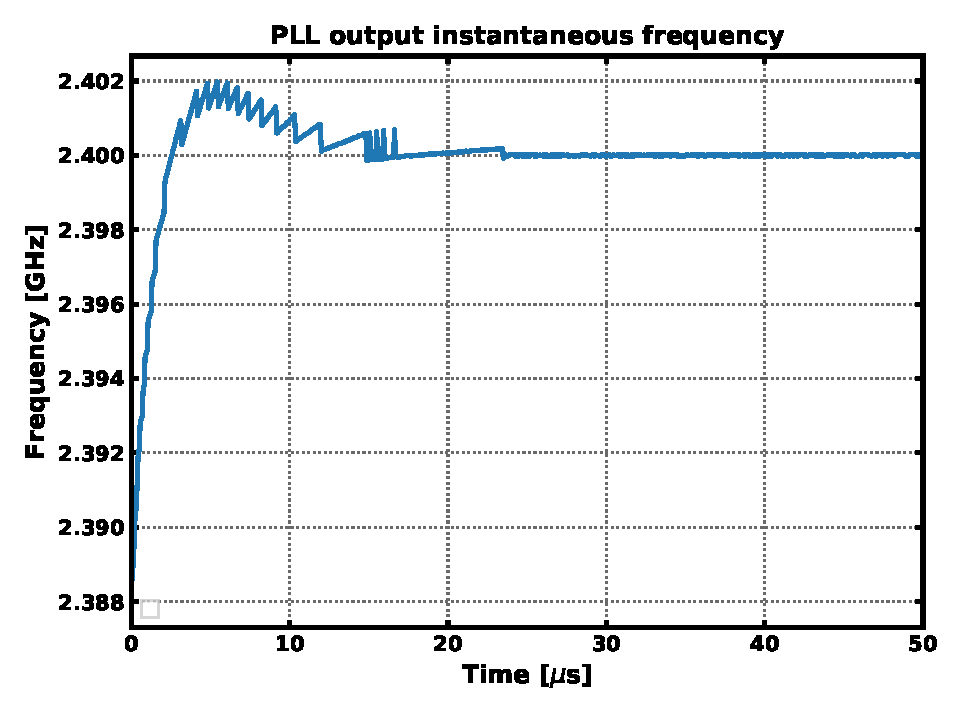
\includegraphics[width=1.0\textwidth, angle=0]{figs/trans_inst_freq.pdf}
	        \caption{ }
	        \label{fig:trans_inst_freq}
	    \end{subfigure}
	    % \caption{Approximate model for ring oscillator inverter delay cell.}
	    \label{fig:trans_sim1}
	    \caption{Simulation with 0.5\% initial frequency error: \textbf{(a)} Loop filter transient response, \textbf{(b)} PLL output instantaneous frequency.}
	\end{figure}

	\begin{figure}[htb!]
	    \centering
	    \begin{subfigure}{0.5\textwidth}
	        \centering
	        \center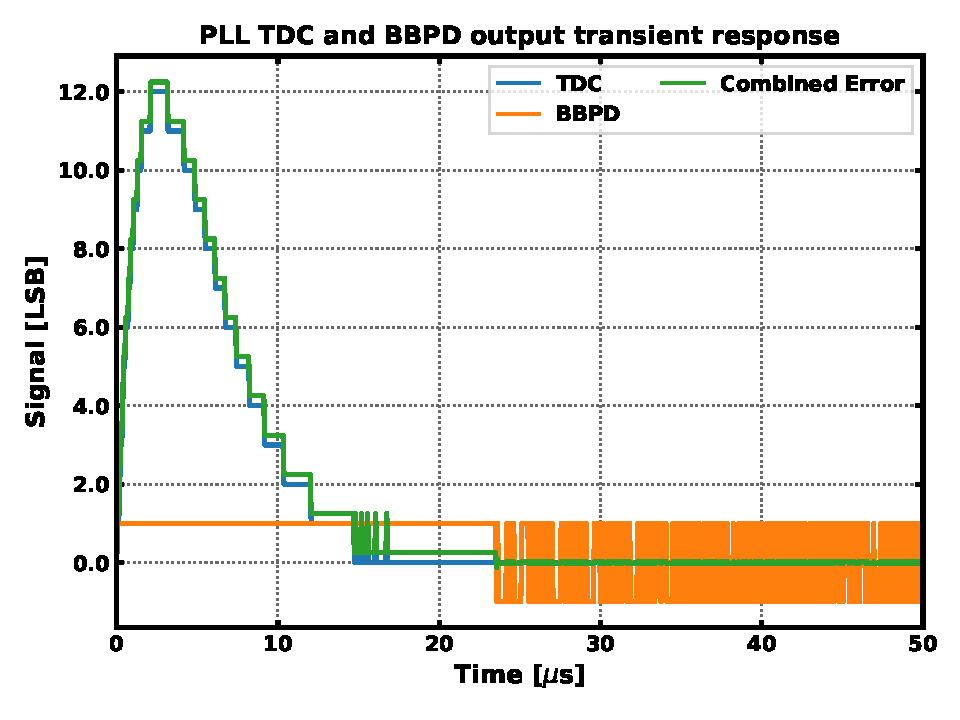
\includegraphics[width=1.0\textwidth, angle=0]{figs/trans_tdc_bbpd.pdf}
	        \caption{ }
	        \label{fig:trans_det}
	    \end{subfigure}%
	    \begin{subfigure}{0.5\textwidth}
	        \centering
	        \center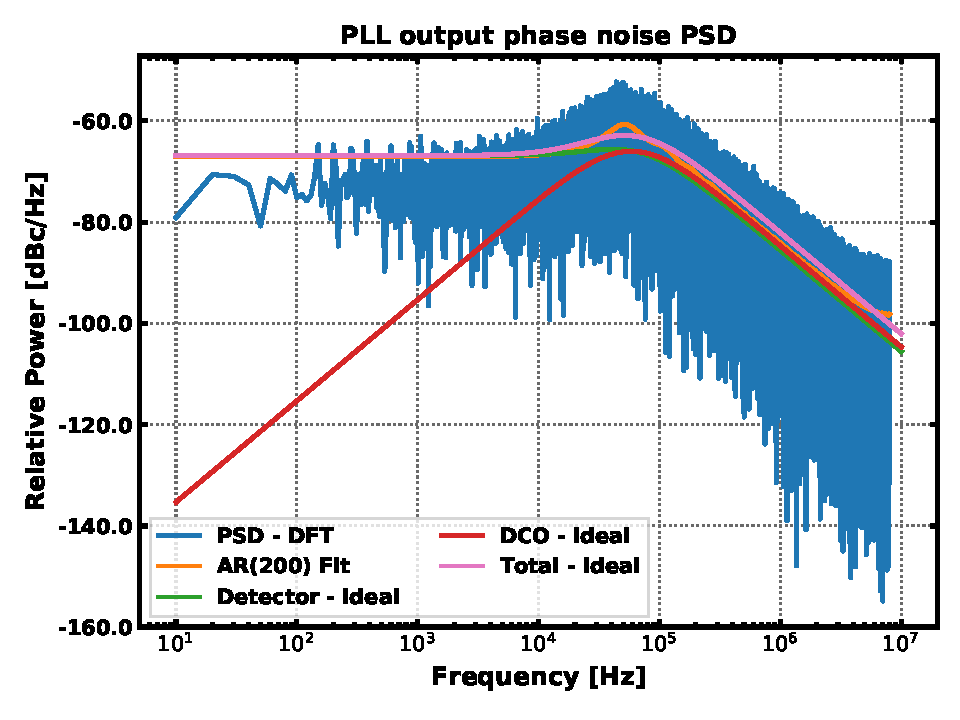
\includegraphics[width=1.0\textwidth, angle=0]{figs/trans_phase_noise.pdf}
	        \caption{ }
	        \label{fig:trans_phase_noise}
	    \end{subfigure}
	    % \caption{Approximate model for ring oscillator inverter delay cell.}
	    \label{fig:trans_sim2}
	    \caption{Simulation with 12 MHz (0.5\%) initial frequency error: \textbf{(a)} BBPD/TDC detector responses, \textbf{(b)} PLL output phase noise power spectrum.}
	\end{figure}
\pagebreak

\subsubsection{Approach 1: Results of Parameter Sweep and Variational Analysis.}
The Monte-Carlo sampling and parametric sweep capabilities of the simulator designed in this work were used to run analysis for effects of variation of DCO gain $K_{DCO}$ and initial frequency error of the PLL. Figure \ref{fig:sweep_kdco} shows a parametric sweep of $K_{DCO}$, with lock time being measured. It is observed that the lock time is nearly flat in the range 7100-21200 Hz/LSB, meaning that there is a tolerance of -2900/+11200 Hz LSB for $K_{DCO}$ about the nominal 10000 Hz/LSB specified. This specification can be utilized in the design of a physical DCO to constrain maximum acceptable variation across PVT. Figure \ref{fig:sweep_finit} demonstrates the simulated effect of initial frequency error on lock time. It is seen that PLL stably locks to the target frequency with an initial frequency error within the interval of $\pm$ 74 MHz from 2.4GHz, implying that the capture range of the PLL is 148 MHz. This specification can be translated into a requirement for initial coarse frequency calibration needed before starting the PLL. Figures \ref{fig:mc_trans} and \ref{fig:mc_hist} are the results of a variation analysis simulation utilizing the Monte-Carlo sampling engine implemented in this work. The simulation was configured to vary $K_{DCO}$ with a standard deviation of 20 \% of the nominal value, and to vary the initial starting frequency with a standard deviation of 60 MHz (2.5 \% of the final frequency). The simulation sample size is 1000. The transient responses from the simulation figure \ref{fig:mc_trans} are all stable, and figure \ref{fig:mc_hist} shows the histogram for measured lock time subject to the described variation. The mean lock time was 19.33 $\mu$s, which correlates well with the estimated 19.34 $\mu$s from the filter design process and meets the 25 $\mu$s lock time set for the PLL. The upper bound for a 99\% confidence interval on the data is 34.75 $\mu$s. A set of extracted parameters from these simulations are in table \ref{simulation_params}. The Monte-Carlo simulations presented here are useful to analyze the range of variation in which the designed PLL can tolerate, as well as determine the expected performance variation, so well informed decisions on a PLL design can be made before moving into transistor level implementation and simulation. 

	\begin{figure}[htb!]
	    \centering
	    \begin{subfigure}{0.5\textwidth}
	        \centering
	        \center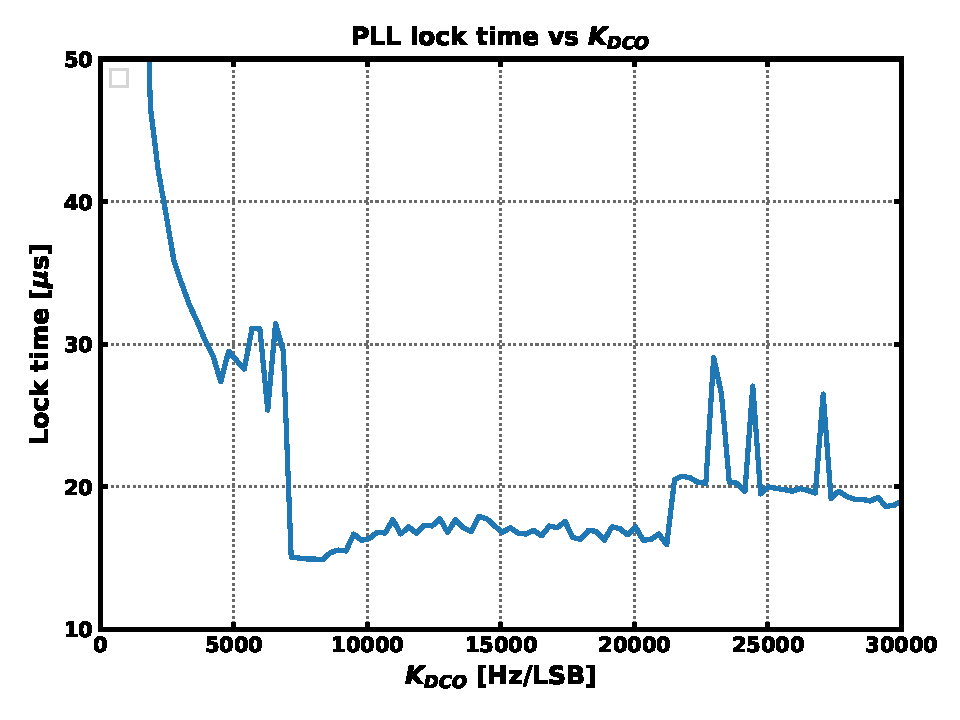
\includegraphics[width=1.0\textwidth, angle=0]{figs/_kdco_sweep.pdf}
	        \caption{ }
	        \label{fig:sweep_kdco}
	    \end{subfigure}%
	    \begin{subfigure}{0.5\textwidth}
	        \centering
	        \center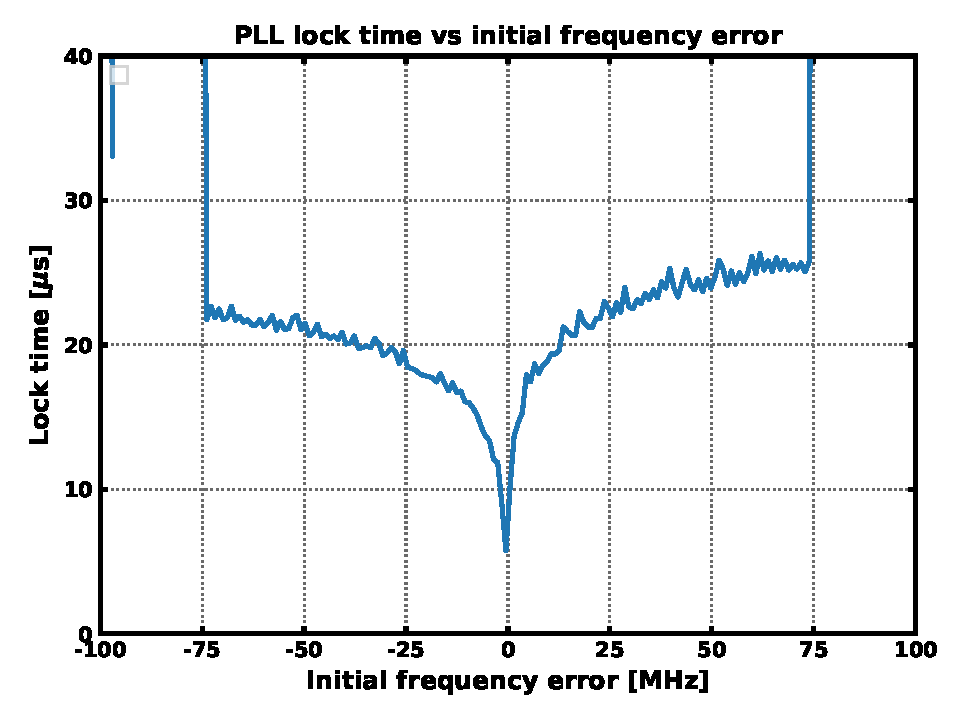
\includegraphics[width=1.0\textwidth, angle=0]{figs/_finit_sweep.pdf}
	        \caption{ }
	        \label{fig:sweep_finit}
	    \end{subfigure}
	    % \caption{Approximate model for ring oscillator inverter delay cell.}
	    \label{fig:sweep_sim}
	    \caption{\textbf{(a)} PLL lock time simulation with KDCO swept, 12 MHz (0.5\%) initial frequency error, \textbf{(b)} PLL lock time simulation with initial frequency error swept.}
	\end{figure}

	\begin{figure}[htb!]
	    \centering
	    \begin{subfigure}{0.5\textwidth}
	        \centering
	        \center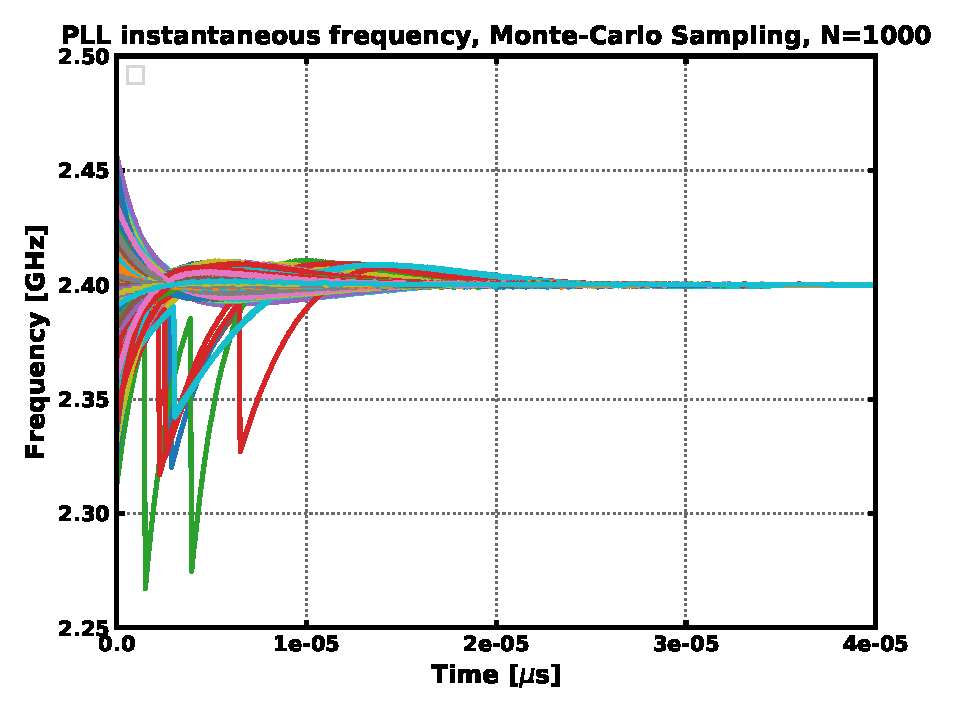
\includegraphics[width=1.0\textwidth, angle=0]{figs/mc_trans.pdf}
	        \caption{ }
	        \label{fig:mc_trans}
	    \end{subfigure}%
	    \begin{subfigure}{0.5\textwidth}
	        \centering
	        \center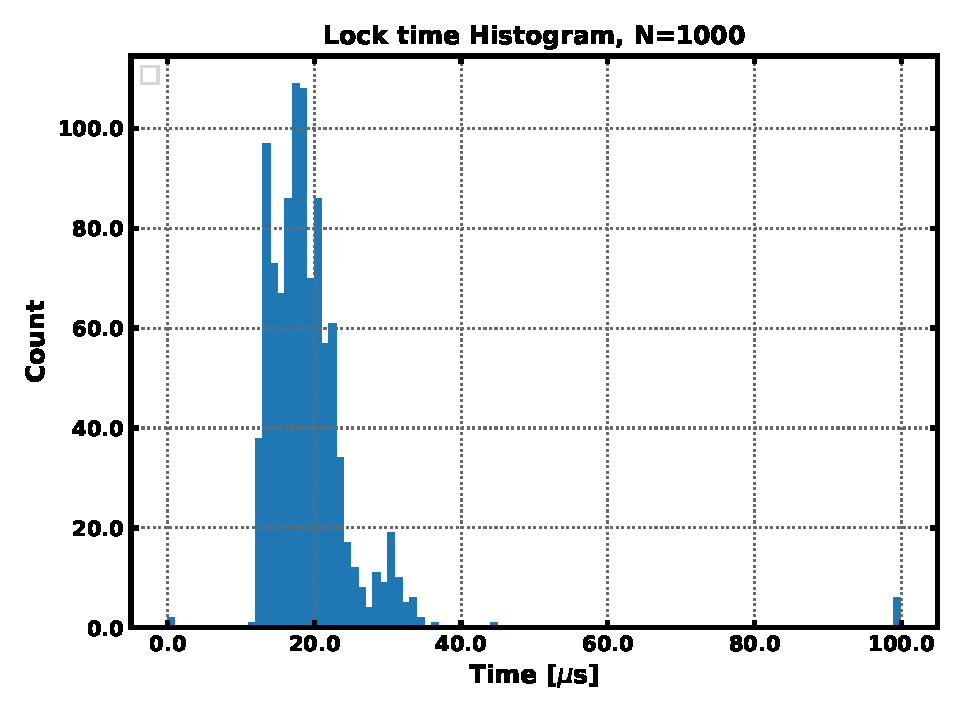
\includegraphics[width=1.0\textwidth, angle=0]{figs/mc_hist.pdf}
	        \caption{ }
	        \label{fig:mc_hist}
	    \end{subfigure}
	    % \caption{Approximate model for ring oscillator inverter delay cell.}
	    \label{fig:mc_sim}
	    \caption{Monte-Carlo simulation with 1000 samples, 20\% RMS deviation in KDCO, and 60 MHz (2.5\%) RMS deviation in initial frequency error \textbf{(a)} Frequency transient responses, \textbf{(b)} Lock time histogram.}
	\end{figure}

\begin{table}[h!]
	\centering
	\def\arraystretch{1.5}		
	\setlength\arrayrulewidth{0.75pt}
	\setlength{\tabcolsep}{1em} % for the horizontal padding
	\begin{tabular}{|l|r|l|}
		\hline 
		\rule[-1ex]{0pt}{2.5ex} \cellcolor{gray!40}\textbf{Parameter} & \cellcolor{gray!40}\textbf{Value} & \cellcolor{gray!40}\textbf{Unit }\\ 
		\hline 
		\rule[-1ex]{0pt}{2.5ex} \textbf{$K_{DCO}$ Tolerance}  & -2900/+11200 & Hz/LSB \\ 
		\hline 
		\rule[-1ex]{0pt}{2.5ex} \textbf{Capture range}  & 148 ($\pm 74$)& MHz\\ 
		\hline 
		\rule[-1ex]{0pt}{2.5ex} \textbf{Mean lock time}  & 19.32769& $\mu$s \\ 
		\hline 
		\rule[-1ex]{0pt}{2.5ex} \textbf{Lock time $\sigma$} & 7.802302 & $\mu$s\\ 
		\hline 
		\rule[-1ex]{0pt}{2.5ex} \textbf{Lock time 99 \% CI upper bound} & 34.75  & $\mu$s\\ 
		\hline 
		\rule[-1ex]{0pt}{2.5ex} \textbf{Residual phase modulation} & $3.374731\times10^{-1}$  & rad$^2$\\ 
		\hline 
	\end{tabular} 

	% \caption{Assigned specifications for branch line hybrid design.}
	% \label{asgn_specs}
	\caption{PLL parameters extracted from variance and parameter sweep simulations.}
	\label{simulation_params}
\end{table}

\subsubsection{Approach 2: Results of Filter Optimization}
The same PLL design has been approached with a second optimization approach utilizing gear switching in the loop filter. The first gear loop filter is optimized for lock speed, using TDC feedback, so high initial frequency and phase errors may be tolerated. After initial lock is achieved with the first filter, the filter is switched gears by changing the digital filter coefficients immediately to a second filter optimized for minimum total phase noise using a BBPD. This combination allow both fast lock and low phase noise. The results of the optimization process are in tables \ref{filter_params_fast_lock} and \ref{filter_params_bbpd_low_noise}, and the optimal digitized filter designs for finite word effects are in table \ref{dig_filter_params_fast}. The total lock time is estimated to be 5.52 $\mu$s. The method for determining number of bits in this work currently assumes the decimal point in the fixed point representation does not change position, so here a total data word size of 20 bits was arrived at, albeit the individual optimization for gear 1 and gear 2 resulted in 10 and 16 bits respectively. This optimization could be improved by considering a filter datapath architecture that handles changing of the decimal position in the loop filter data words during gear switching.

\begin{table}[h!]
	\centering
	\def\arraystretch{1.5}		
	\setlength\arrayrulewidth{0.75pt}
	\setlength{\tabcolsep}{1em} % for the horizontal padding
	\begin{tabular}{|l|r|l|}
		\hline 
		\rule[-1ex]{0pt}{2.5ex} \cellcolor{gray!40}\textbf{Parameter} & \cellcolor{gray!40}\textbf{Value} & \cellcolor{gray!40}\textbf{Unit }\\ 
		\hline 
		\rule[-1ex]{0pt}{2.5ex} \textbf{$K$}  & $2.982197\times10^{12}$ &  \\
		\hline 
		\rule[-1ex]{0pt}{2.5ex} \textbf{$K_i$}  & $2.982197\times10^{8}$ &  \\
		\hline 
		\rule[-1ex]{0pt}{2.5ex} \textbf{$K_p$}  & $2.115052\times10^{2}$ &  \\
		\hline 
		\rule[-1ex]{0pt}{2.5ex} \textbf{$f_z$} & $2.244064\times10^5$ & Hz\\
		\hline 
		\rule[-1ex]{0pt}{2.5ex} \textbf{$b_0$}  & $2.3014397180\times10^2$  &\\
		\hline 
		\rule[-1ex]{0pt}{2.5ex} \textbf{$b_1$}  & $-2.1150524223\times10^2$  & \\
		\hline 
		\rule[-1ex]{0pt}{2.5ex} \textbf{$a_0$}  & $1.0\times10^0$  &\\ 
		\hline 
		\rule[-1ex]{0pt}{2.5ex} \textbf{$a_1$}  & $-1.0\times10^0$  & \\
		\hline 
		\rule[-1ex]{0pt}{2.5ex} \textbf{$a_2$}  & $0.0\times10^0$  & \\
		\hline 
		\rule[-1ex]{0pt}{2.5ex} Estimated bandwidth & $5.333423\times10^5$ & Hz \\
		\hline 
		\rule[-1ex]{0pt}{2.5ex} Estimated lock time & $4.527067\times10^{-6}$ & seconds \\
		\hline 
	\end{tabular} 
	% \caption{Assigned specifications for branch line hybrid design.}
	% \label{asgn_specs}
	\caption{PLL parameters determined from filter design and optimization process for fast lock speed with TDC feedback.}
	\label{filter_params_fast_lock}
\end{table}   

\begin{table}[h!]
	\centering
	\def\arraystretch{1.5}		
	\setlength\arrayrulewidth{0.75pt}
	\setlength{\tabcolsep}{1em} % for the horizontal padding
	\begin{tabular}{|l|r|l|}
		\hline 
		\rule[-1ex]{0pt}{2.5ex} \cellcolor{gray!40}\textbf{Parameter} & \cellcolor{gray!40}\textbf{Value} & \cellcolor{gray!40}\textbf{Unit }\\ 
		\hline 
		\rule[-1ex]{0pt}{2.5ex} \textbf{$K$}  & $5.325862\times12^{12}$ &  \\
		\hline 
		\rule[-1ex]{0pt}{2.5ex} \textbf{$K_i$}  & $1.271456\times10^{10}$ &  \\
		\hline 
		\rule[-1ex]{0pt}{2.5ex} \textbf{$K_p$}  & $1.101813\times10^{4}$ &  \\
		\hline 
		\rule[-1ex]{0pt}{2.5ex} \textbf{$f_z$} & $1.836596\times10^5$ & Hz\\
		\hline 
		\rule[-1ex]{0pt}{2.5ex} \textbf{$b_0$}  & $1.1812790734\times10^4$  &\\
		\hline 
		\rule[-1ex]{0pt}{2.5ex} \textbf{$b_1$}  & $-1.1018130778\times10^4$  & \\
		\hline 
		\rule[-1ex]{0pt}{2.5ex} \textbf{$a_0$}  & $1.0\times10^0$  &\\ 
		\hline 
		\rule[-1ex]{0pt}{2.5ex} \textbf{$a_1$}  & $-1.0\times10^0$  & \\ 
		\hline 
		\rule[-1ex]{0pt}{2.5ex} \textbf{$a_2$}  & $0.0\times10^0$  & \\ 
		\hline 
		\rule[-1ex]{0pt}{2.5ex} \textbf{$K_{bb}$}  & $1.0\times10^0$  & \\ 
		\hline 
		\rule[-1ex]{0pt}{2.5ex} Estimated bandwidth & $9.117332\times10^5$ & Hz \\
		\hline 
		\rule[-1ex]{0pt}{2.5ex} Estimated lock time & $9.978130\times10^{-7}$ & seconds \\
		\hline 
	\end{tabular} 
	% \caption{Assigned specifications for branch line hybrid design.}
	% \label{asgn_specs}
	\caption{PLL parameters determined from filter design and optimization process for minimum phase noise with BBPD.}
	\label{filter_params_bbpd_low_noise}
\end{table}   

\begin{table}[h!]
	\centering
	\def\arraystretch{1.5}		
	\setlength\arrayrulewidth{0.75pt}
	\setlength{\tabcolsep}{1em} % for the horizontal padding
	\begin{tabular}{|l|r|r|l|}
		\hline 
		\rule[-1ex]{0pt}{2.5ex} \cellcolor{gray!40}\textbf{Parameter} & \cellcolor{gray!40}\textbf{Value} & \cellcolor{gray!40}\textbf{Value (digital) } & \cellcolor{gray!40}\textbf{Value Error}\\ 
		\hline 
		\rule[-1ex]{0pt}{2.5ex} Total dataword bits  & 20 & & \\ 
		\hline 
		\rule[-1ex]{0pt}{2.5ex} Sign bits  & 1 & & \\ 
		\hline 
		\rule[-1ex]{0pt}{2.5ex} Integer bits & 8 & & \\ 
		\hline 
		\rule[-1ex]{0pt}{2.5ex} Fractional bits  & 11 & & \\ 
		\hline 
		\rule[-1ex]{0pt}{2.5ex} \textbf{$b_0$} {\color{red} (gear 1)} & $2.301440\times10^2$ & \texttt{0b01110011000100100111}  & $+7.116930\times10^{-5}$\\
		\hline 
		\rule[-1ex]{0pt}{2.5ex} \textbf{$b_1$} {\color{red} (gear 1)} & $-2.115054\times10^2$ & \texttt{0b11110110001111110101}  & $-1.288619\times10^{-4}$\\
		\hline 
		\rule[-1ex]{0pt}{2.5ex} \textbf{$a_0$} {\color{red} (gear 1)} & $1.0\times10^0$ & \texttt{0b00000000100000000000} & $0.0\times10^0$ \\ 
		\hline 
		\rule[-1ex]{0pt}{2.5ex} \textbf{$a_1$} {\color{red} (gear 1)} & $-1.0\times10^0$ & \texttt{0b11111111100000000000} & $0.0\times10^0$ \\ 
		\hline 
		\rule[-1ex]{0pt}{2.5ex} \textbf{$a_2$} {\color{red} (gear 1)} & $0.0\times10^0$ & \texttt{0b00000000000000000000} & $0.0\times10^0$ \\ 
		\hline 
		\rule[-1ex]{0pt}{2.5ex} \textbf{$K_{bb}$} {\color{red} (gear 1)} & $0.0\times10^0$ & \texttt{0b00000000000000000000} & $0.0\times10^0$ \\ 
		\hline 
		\rule[-1ex]{0pt}{2.5ex} \textbf{$b_0$} {\color{blue} (gear 2)} & $8.899902\times10^0$ & \texttt{0b00000100011100110011}  & $+4.616306\times10^{-5}$\\
		\hline 
		\rule[-1ex]{0pt}{2.5ex} \textbf{$b_1$} {\color{blue} (gear 2)} & $-8.301270\times10^0$ & \texttt{0b11111011110110010111}  & $-1.168639\times10^{-4}$\\
		\hline 
		\rule[-1ex]{0pt}{2.5ex} \textbf{$a_0$} {\color{blue} (gear 2)} & $1.0\times10^0$ & \texttt{0b00000000100000000000} & $0.0\times10^0$ \\ 
		\hline 
		\rule[-1ex]{0pt}{2.5ex} \textbf{$a_1$} {\color{blue} (gear 2)} & $-1.0\times10^0$ & \texttt{0b11111111100000000000} & $0.0\times10^0$ \\ 
		\hline 
		\rule[-1ex]{0pt}{2.5ex} \textbf{$a_2$} {\color{blue} (gear 2)} & $0.0\times10^0$ & \texttt{0b00000000000000000000} & $0.0\times10^0$ \\ 
		\hline 
		\rule[-1ex]{0pt}{2.5ex} \textbf{$K_{bb}$} {\color{blue} (gear 2)} & $1.0\times10^0$ & \texttt{0b00000000100000000000} & $1\times10^0$ \\ 
		\hline 
	\end{tabular} 
	% \caption{Assigned specifications for branch line hybrid design.}
	% \label{asgn_specs}
	\caption{Loop filter parameters after digitization and optimization for data word length, gear 1 and gear 2.}
	\label{dig_filter_params_fast}
\end{table}  

\subsubsection{Approach 2: Results of Transient and Phase Noise Simulation}
It is observed that the fast lock gear converges the PLL to steady state in approximately 6 $\mu$s as seen in the transient step simulation in figures \ref{fig:trans_lf_fast} and \ref{fig:trans_inst_freq_fast}, where an initial frequency error of 0.5\% {12 MHz} is used. Figure \ref{fig:trans_det_fast} shows the output of the TDC and BBPD, it is seen that BBPD feedback has a high density at approximately 11 $\mu$s, implicating steady state conditions. Finally, the computed phase noise spectrum of figure \ref{fig:trans_phase_noise_fast} demonstrates that there is some discrepancy between the ideal designed response and that simulated, albeit the bandwidth appears correct. The phase noise spectrum discrepancy is likely due to the model used in the optimization for the BBPD, which uses a linearized model of the BBPD with only idealized DCO and detector noise considered. This does not accurately account for all quantization and discretization emergent behaviors in the discrete time behavioral simulation possibly being manifested here. 

	\begin{figure}[htb!]
	    \centering
	    \begin{subfigure}{0.5\textwidth}
	        \centering
	        \center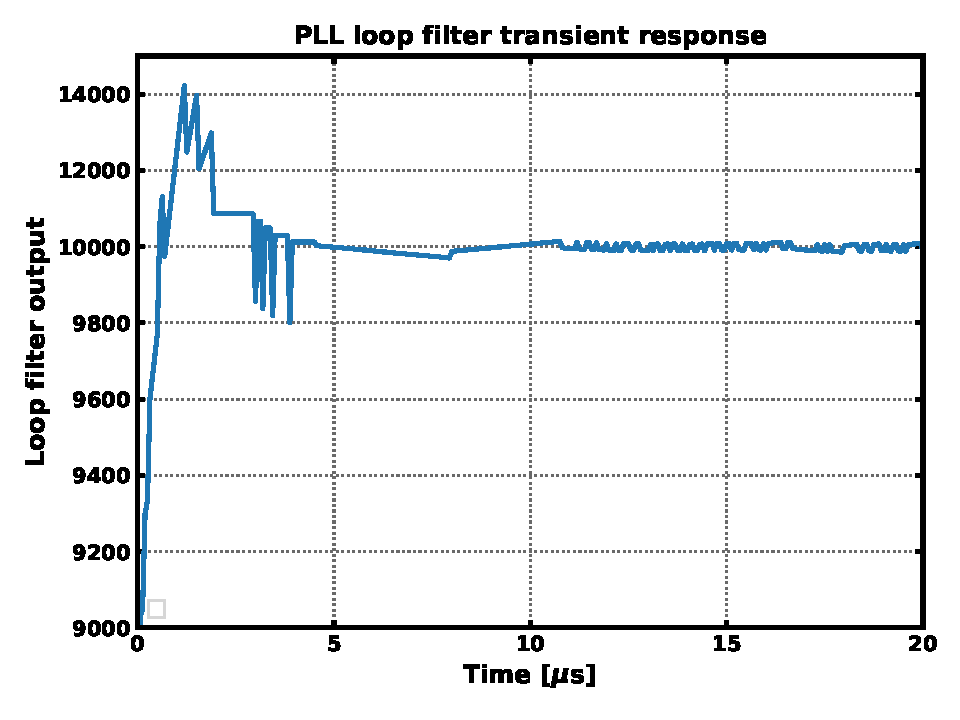
\includegraphics[width=1.0\textwidth, angle=0]{figs/trans_loop_filter_fast.pdf}
	        \caption{ }
	        \label{fig:trans_lf_fast}
	    \end{subfigure}%
	    \begin{subfigure}{0.5\textwidth}
	        \centering
	        \center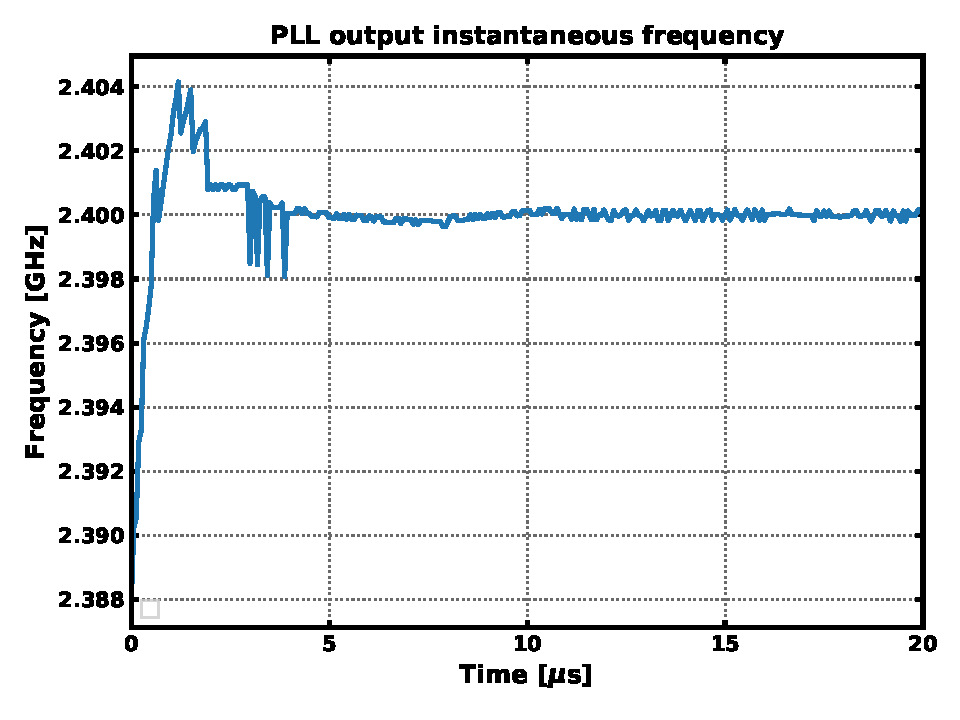
\includegraphics[width=1.0\textwidth, angle=0]{figs/trans_inst_freq_fast.pdf}
	        \caption{ }
	        \label{fig:trans_inst_freq_fast}
	    \end{subfigure}
	    % \caption{Approximate model for ring oscillator inverter delay cell.}
	    \label{fig:trans_sim1_fast}
	    \caption{Simulation with 0.5\% initial frequency error: \textbf{(a)} Loop filter transient response, \textbf{(b)} PLL output instantaneous frequency.}
	\end{figure}

	\begin{figure}[htb!]
	    \centering
	    \begin{subfigure}{0.5\textwidth}
	        \centering
	        \center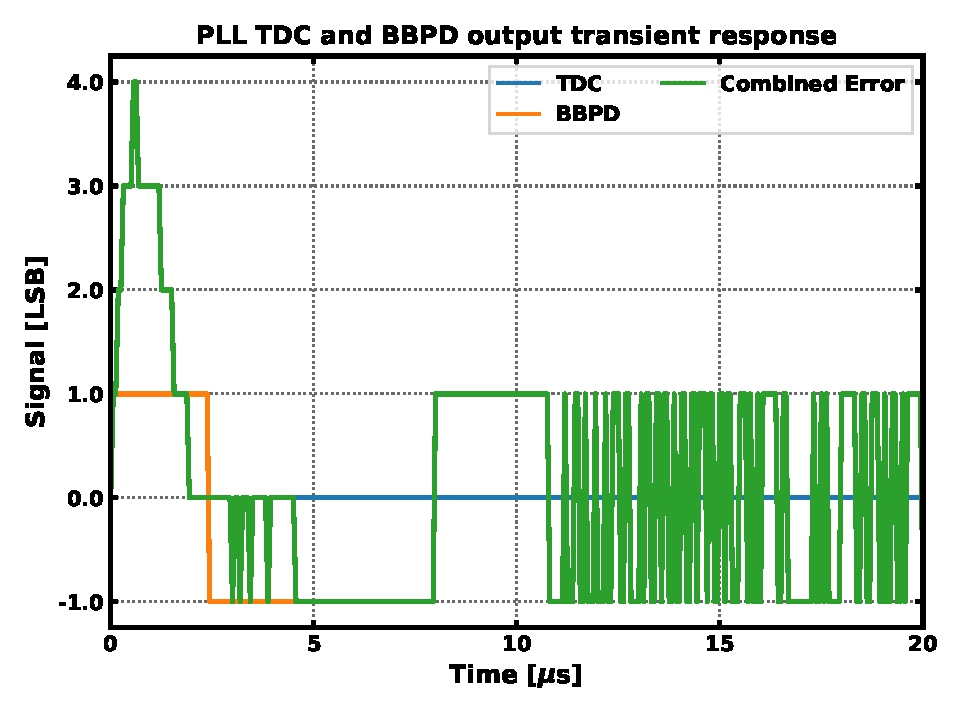
\includegraphics[width=1.0\textwidth, angle=0]{figs/trans_tdc_bbpd_fast.pdf}
	        \caption{ }
	        \label{fig:trans_det_fast}
	    \end{subfigure}%
	    \begin{subfigure}{0.5\textwidth}
	        \centering
	        \center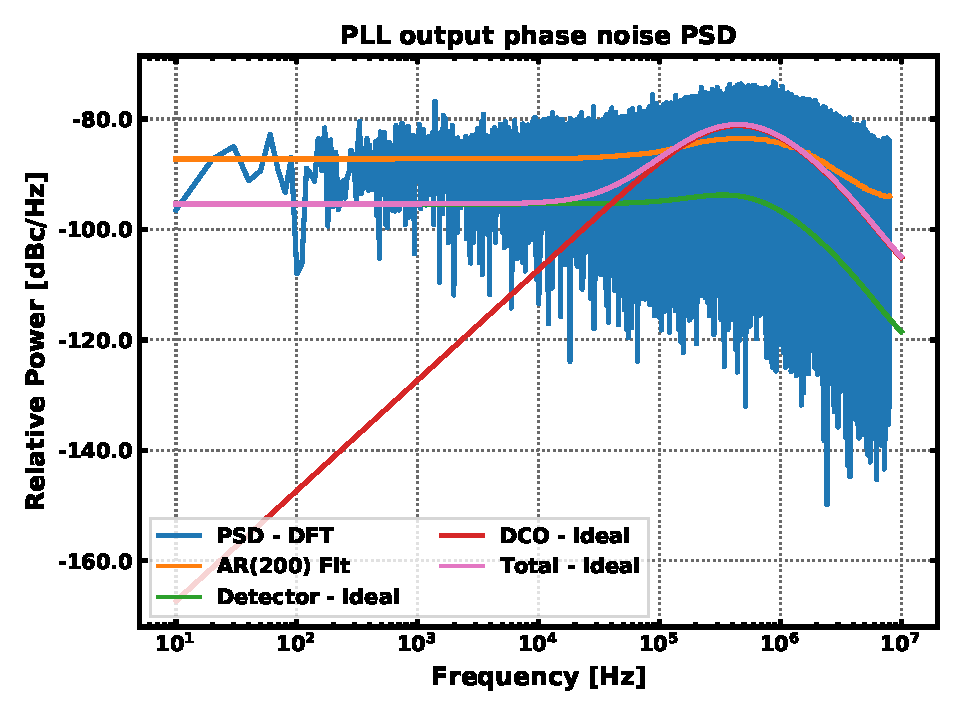
\includegraphics[width=1.0\textwidth, angle=0]{figs/trans_phase_noise_fast.pdf}
	        \caption{ }
	        \label{fig:trans_phase_noise_fast}
	    \end{subfigure}
	    % \caption{Approximate model for ring oscillator inverter delay cell.}
	    \label{fig:trans_sim2_fast}
	    \caption{Simulation with 12 MHz (0.5\%) initial frequency error: \textbf{(a)} BBPD/TDC detector responses, \textbf{(b)} PLL output phase noise power spectrum.}
	\end{figure}
\subsubsection{Approach 2: Results of Parameter Sweep and Variational Analysis}
The same parameter sweeps for $K_{DCO}$ and initial frequency error of approach 1 were applied here. In figures \ref{fig:sweep_kdco_fast} and \ref{fig:sweep_finit_fast}, the results of these sweeps are shown. The loop filter gear switching mechanism as modeled in the simulation waits a fixed time interval before switching gears, in this case chosen to be 2.0 times the estimated lock time given in table \ref{filter_params_fast_lock}. This interval has provided sufficient settling within the simulated parameter range of $K_{DCO}$ and initial frequency error that lock time stability is observed under most conditions, except under high offset for $K_{DCO}$ and initial frequency error. It was established for this simulation results that tolerance range for $K_{DCO}$ is -6950/+9750 Hz/LSB from the nominal 10000 Hz/LSB value, and the capture range is 168 MHz. Figures \ref{fig:mc_trans_fast} and \ref{fig:mc_hist_fast} demonstrate a variational simulation of the PLL using Monte-Carlo sampling, with 1000 samples. The simulation was configured to vary $K_{DCO}$ with a standard deviation of 20 \% of the nominal value, and to vary the initial starting frequency with a standard deviation of 60 MHz (2.5 \% of the final frequency). It was observed that the PLL stably locked for all simulation instances, a mean lock time of 5.96 $\mu$s was achieved. This value correlates well with the estimate of 5.52 $\mu$s from the filter design process. The upper bound for a 99\% confidence interval of lock time is 11.625 $\mu$s, thus meeting the 25$\mu$s lock time specification with considerable margin. The extracted PLL performance parameters from these simulations of this gear-switching PLL is in table \ref{simulation_params_fast}. 
	\begin{figure}[htb!]
	    \centering
	    \begin{subfigure}{0.5\textwidth}
	        \centering
	        \center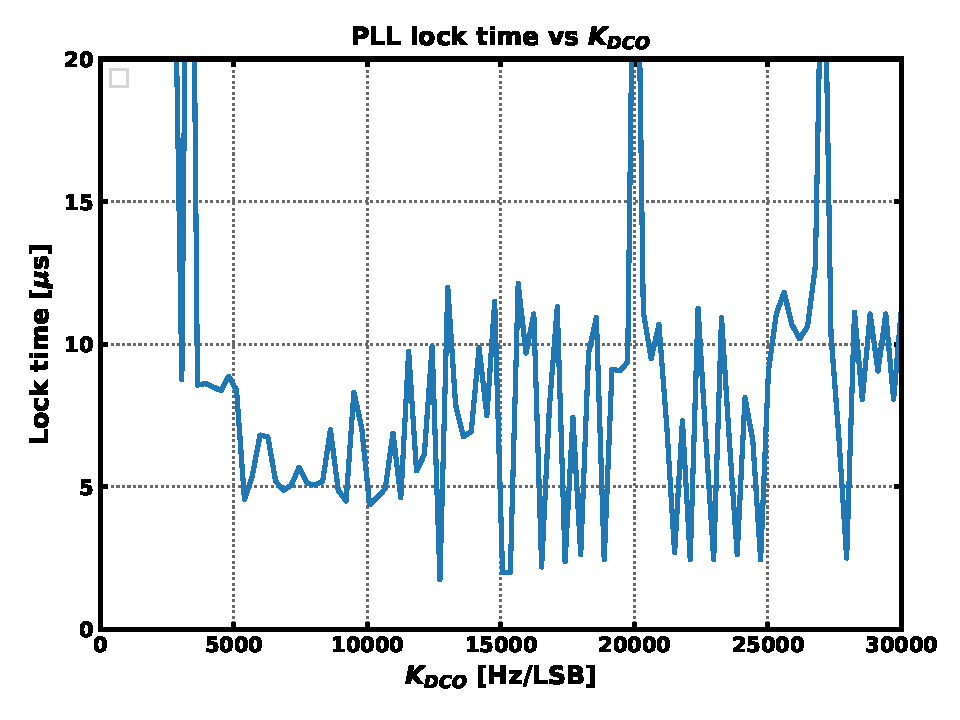
\includegraphics[width=1.0\textwidth, angle=0]{figs/_kdco_sweep_fast.pdf}
	        \caption{ }
	        \label{fig:sweep_kdco_fast}
	    \end{subfigure}%
	    \begin{subfigure}{0.5\textwidth}
	        \centering
	        \center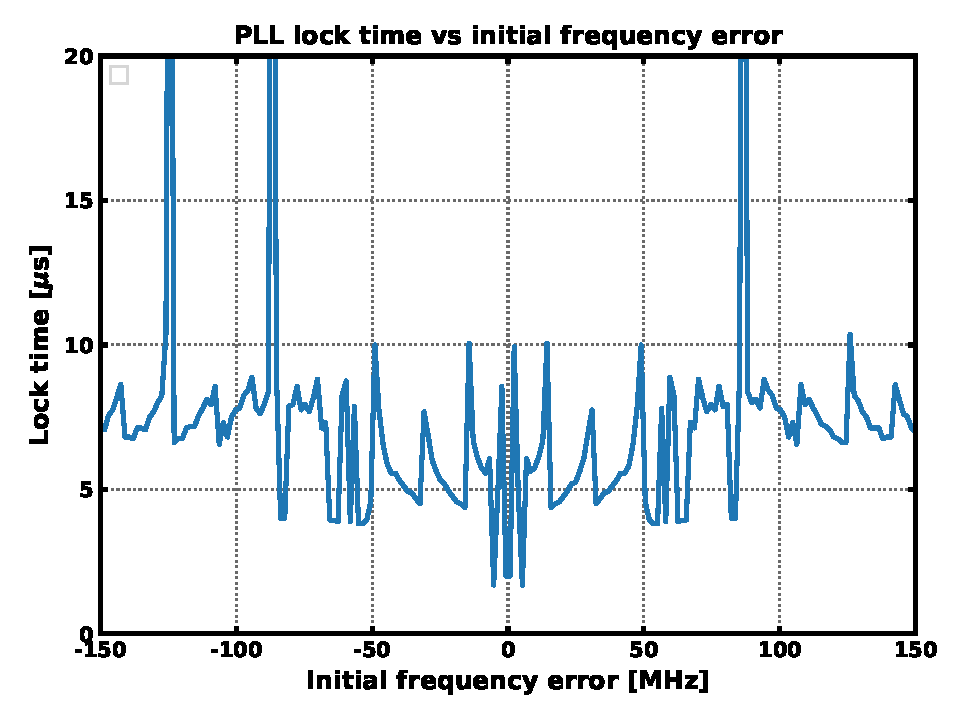
\includegraphics[width=1.0\textwidth, angle=0]{figs/finit_sweep_fast.pdf}
	        \caption{ }
	        \label{fig:sweep_finit_fast}
	    \end{subfigure}
	    % \caption{Approximate model for ring oscillator inverter delay cell.}
	    \label{fig:sweep_sim_fast}
	    \caption{\textbf{(a)} PLL lock time simulation with KDCO swept, 12 MHz (0.5\%) initial frequency error, \textbf{(b)} PLL lock time simulation with initial frequency error swept.}
	\end{figure}

	\begin{figure}[htb!]
	    \centering
	    \begin{subfigure}{0.5\textwidth}
	        \centering
	        \center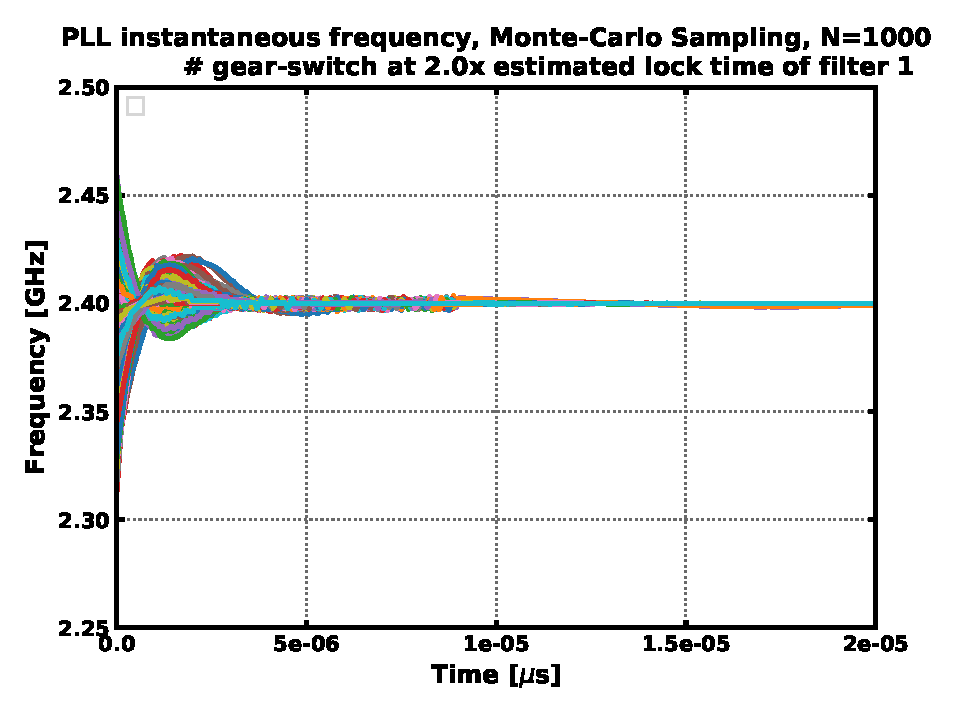
\includegraphics[width=1.0\textwidth, angle=0]{figs/mc_trans_2x.pdf}
	        \caption{ }
	        \label{fig:mc_trans_fast}
	    \end{subfigure}%
	    \begin{subfigure}{0.5\textwidth}
	        \centering
	        \center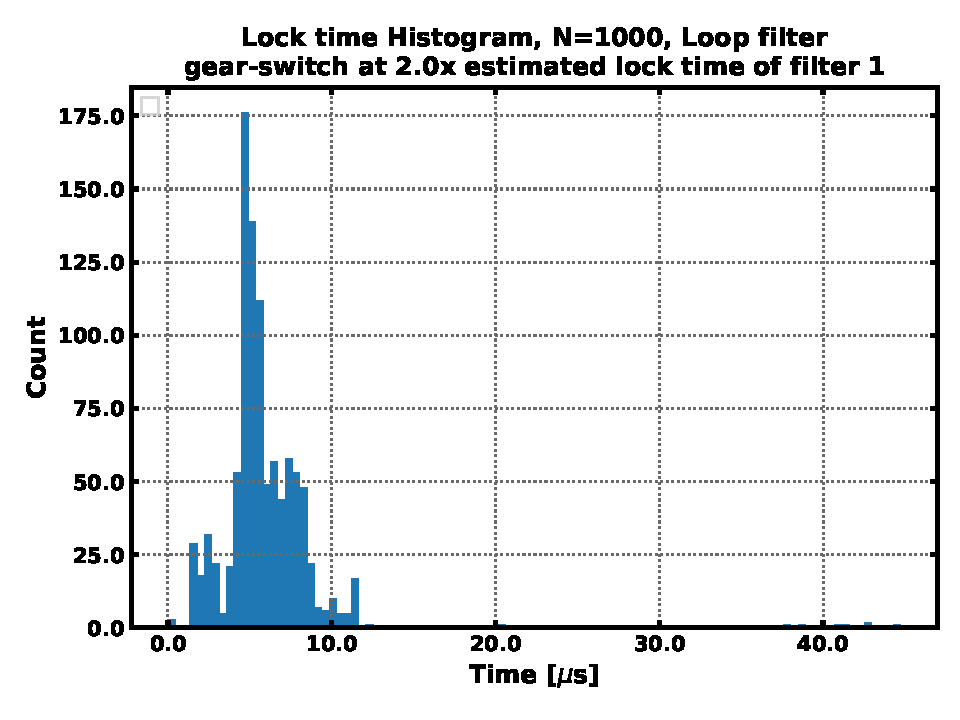
\includegraphics[width=1.0\textwidth, angle=0]{figs/mc_hist_fast_2x.pdf}
	        \caption{ }
	        \label{fig:mc_hist_fast}
	    \end{subfigure}
	    % \caption{Approximate model for ring oscillator inverter delay cell.}
	    \label{fig:mc_sim_fast}
	    \caption{Monte-Carlo simulation with 1000 samples, 20\% RMS deviation in KDCO, and 60 MHz (2.5\%) RMS deviation in initial frequency error \textbf{(a)} Frequency transient responses, \textbf{(b)} Lock time histogram.}
	\end{figure}

\begin{table}[h!]
	\centering
	\def\arraystretch{1.5}		
	\setlength\arrayrulewidth{0.75pt}
	\setlength{\tabcolsep}{1em} % for the horizontal padding
	\begin{tabular}{|l|r|l|}
		\hline 
		\rule[-1ex]{0pt}{2.5ex} \cellcolor{gray!40}\textbf{Parameter} & \cellcolor{gray!40}\textbf{Value} & \cellcolor{gray!40}\textbf{Unit }\\ 
		\hline 
		\rule[-1ex]{0pt}{2.5ex} \textbf{$K_{DCO}$ Tolerance}  & -6950/+9750 & Hz/LSB \\
		\hline 
		\rule[-1ex]{0pt}{2.5ex} \textbf{Capture range}  & 168 ($\pm 84$)& MHz\\ 
		\hline 
		\rule[-1ex]{0pt}{2.5ex} \textbf{Mean lock time}  & 5.961688& $\mu$s \\
		\hline 
		\rule[-1ex]{0pt}{2.5ex} \textbf{Lock time $\sigma$} & 3.611130 & $\mu$s\\ 
		\hline 
		\rule[-1ex]{0pt}{2.5ex} \textbf{Lock time 99 \% CI upper bound} & 11.625  & $\mu$s\\
		\hline 
		\rule[-1ex]{0pt}{2.5ex} \textbf{Residual phase modulation} & $4.367535\times10^{-2}$ & rad$^2$\\ 
		\hline 
	\end{tabular} 

	% \caption{Assigned specifications for branch line hybrid design.}
	% \label{asgn_specs}
	\caption{PLL parameters extracted from variance and parameter sweep simulations.}
	\label{simulation_params_fast}
\end{table}
\pagebreak
\subsubsection{Results Comparison of Design Approaches}
A comparison of the two design approaches shows that the PLL utilizing the gear switching results in a superior result using the design automation framework of this work. The usage of gear switching results in lower phase noise than approach 1, with total phase noise power (residual phase modulation) of 4.36$\times 10^{-2}$ rad$^2$ versus 3.37$\times 10^{-1}$ rad$^2$. Additionally, the lock time is significantly lower in the PLL with gear switching, at an average of 5.96 $\mu$s versus 19.32 $\mu$s. Therefore it has been shown that this framework offers the capability to design gear-switching PLLs with performance advantages to static loop filter PLL designs.

	% \begin{figure}[htb!]
	% 	\center\includegraphics[width=1.0\textwidth, angle=0]{figs/x.pdf}
	% 	\caption{Transient simulation of optimal design.}
	% 	\label{fig:des_ex_trans}
	% \end{figure}
	% \FloatBarrier

	% \begin{figure}[htb!]
	% 	\center\includegraphics[width=1.0\textwidth, angle=0]{figs/x.pdf}
	% 	\caption{Variation Simulation for KDCO.}
	% 	\label{fig:var_lock}
	% \end{figure}
	% \FloatBarrier

	% \begin{figure}[htb!]
	% 	\center\includegraphics[width=1.0\textwidth, angle=0]{figs/x.pdf}
	% 	\caption{Phase noise.}
	% 	\label{fig:Simulated phase noise.}
	% \end{figure}
	% \FloatBarrier

	% stability criteria - Jurys' stability criteria abs(a0) l.t. a2 for second order z-transfer \cite{xiu_li_meiners_padakanti_2004}
	% - Not phase margin based in optimization, can make stable by using stable choice of PI controller (two poles only) - poles should be in unit circle...
\FloatBarrier
\subsection{Comparison to Existing Solutions}
Due to the relative youth of all digital PLL design, and discontinuity between the continuous theory of analog PLL and digital PLL design, a smaller body of work exist pertaining to the loop filters for exclusively ADPLLs. Of the existing literature, the majority design approaches utilize discrete-time transformed PI-controller loop filters with either bang-bang phase detectors \cite{zanuso_2009}\cite{xu_abidi_2017}\cite{kratyuk_2007}\cite{safwat_ghoneima_ismail_2011} or phase-frequency detectors \cite{kumm_klingbeil_zipf_2010}\cite{chau_chen_2009}. This work takes a similar approach to the aforementioned existing works, focusing on a fixed filter architecture to limit the scope of the problem at hand, and also uses a bang-bang phase detector in its PLL architecture. This work, though, uniquely considers the optimization of digital loop filter design to use a TDC and BBPD in conjunction. Also, the approach to filter design here, which is through numerical methods to find an optimal configuration, differs from the other works that largely focus on closed-form mathematical analysis. The usage of numerical methods has allowed for implementation in this work of (a) full automation of the loop filter design process, including generation of optimal digitized filter coefficients, and (b) automatic verification through the simulator integrated into this filter design framework. These aspects of this work reduces overall implementation work for the PLL designer, and are not paralleled by any existing literature or openly available code bases. 

The criteria and motivation for loop design varies across the surveyed works. Of the surveyed works, several \cite{kratyuk_2007}\cite{kumm_klingbeil_zipf_2010}\cite{chau_chen_2009}\cite{safwat_ghoneima_ismail_2011} do not consider optimization for phase noise as this work principally does, but rather consider stability/phase margin \cite{kratyuk_2007}\cite{kumm_klingbeil_zipf_2010}\cite{safwat_ghoneima_ismail_2011}, lock time \cite{chau_chen_2009}\cite{safwat_ghoneima_ismail_2011} and even approach simplicity \cite{kumm_klingbeil_zipf_2010}. The methods that consider optimization of phase noise \cite{zanuso_2009}\cite{xu_abidi_2017} both provide a similar model of PLL dynamics based on a linearized model of the bang-bang phase detector. The design methods of the latter two works are presented with closed-form mathematical theory, using closed loop transfer function modeling to estimate phase noise from BBPD and oscillator contributions. The simulation results presented and the demonstration of correlation of their model to measurement in \cite{xu_abidi_2017}, which correlate better than that seen in this work, perhaps imply these methods provide for better optimization of BBPD-PLL phase noise than this work. The simulation methods used in those works are not described, so it is unknown if the simulations capture the presence of discrete-time and quantization-related emergent behaviors not in with their linearized PLL models. In the case of \cite{xu_abidi_2017} it appears that the loop filter is treated to be analog in nature, which differs from this work. Since the simulator used in this work accounts for full discrete-time and quantization effects, perhaps this may explain some level of observed discrepancy in the model versus simulation results compared to that in literature. 

Few of the existing works consider the implementation of the loop filter design into digital hardware, rather just provide continuous valued coefficients for the filter designs. Of those surveyed, only \cite{kumm_klingbeil_zipf_2010} provides an analysis for quantization noise in terms of spurious-free dynamic range SFDR out of the loop filter design, but lacks the connection to output phase noise. This work uniquely considers (a) the impact of quantization of the digitized filter design, in terms of filter accuracy and output phase noise, and (b) attempts to optimize the digital implementation of the filter in terms of number of bits the various components of the filter (i.e. filter coefficients, multipliers, adders) are implemented with for complexity and performance.

A final advantage of this work not observed in the surveyed literature is the integrated PLL simulator with Monte-Carlo sampling which allows for verification of the designed loop filter with accurate modeling of time-discretization and digital quantization effects. This allows for lock time, phase noise and stability to be verified on the design to ensure it meets the designer's requirements before moving onto testing with transistor level implementations and testing.

\subsection{Design Choices and Areas of Improvement}
In the design of the filter optimization in this framework for phase noise, a choice was made to only consider phase noise components resulting from detector (TDC and BBPD) noise and oscillator noise. This choice has been motivated from the reasoning that other PLL noise components, being loop filter and divider noise, can be reduced below that of these components with relative ease. In the case of the loop filter noise in a digital PLL, noise results from quantization within the filter implementation are connected with finite word effects. It shown in section \ref{lf_quant_noise_opt} that the quantization noise can be reduced considerably by increasing the number of bits used to represent data in the digital filter representation. As it was seen in figure \ref{fig:ex_pll_pn_comps}, the detector phase noise referred to the PLL output in the PLL architecture of this work is low pass with higher order roll than the TDC, thus a sufficient number of bits utilized in the loop filter implementation data words will reduce all output-referred loop filter noise components below detector noise. An optimizer was accordingly implemented in this work to select the optimal number of bits automatically for loop filter noise to be insignificant. In the case of divider noise, it is seen in the theory of section \ref{final_pn_model} in equations \ref{eq:tdc_pn_psd} and \ref{eq:div_pn_psd} that the detector noise (in this case TDC) and divider noise PSD referred to the PLL output both have a frequency dependence proportional to the closed loop PLL response, i.e. $\propto\hat{\mathrm{T}}(s)$. As demonstrated in appendix \ref{div_noise_constraint}, by constraining the output PSD of the divider to be below detector, it is found that the maximum allowed divider RMS jitter $\sigma_{tn_{div}}$ is in equation \ref{eq:max_div_jitter}, for a TDC with with M steps per reference cycle. This is observed to be equal to the time resolution of the detector, in the case of the TDC $\Delta t_{step_{TDC}}$. This shows that the divider jitter requirement is rather loose, for example with a 10 MHz reference frequency and a 1000-step resolution TDC, the maximum RMS jitter limit is 100 ps. 
\begin{equation}\label{eq:max_div_jitter}
		\sigma_{tn_{div}} < \frac{1}{\mathrm{M}f_{ref}} = \Delta t_{step_{TDC}}
\end{equation}

A further choice in the modeling and optimization of phase noise in this work was to only utilize $\propto f^{-2}$ components of oscillator phase noise from the Leeson model discussed in section \ref{dco_noise}, ignoring flicker frequency ($\propto f^{-1}$) components. The rationale for the exclusion of flicker noise components was that it is expected that flicker components of the reference oscillator will be significantly larger than the DCO contributions. Analyzing the PLL phase noise sensitivity transfer functions of section \ref{ntfs} shows that divider and reference noise is transferred to PLL output with sensitivity N$\hat{\mathrm{T}}(s)$, and DCO noise with 1-$\hat{\mathrm{T}}(s)$. The normalized PLL transfer function $\hat{\mathrm{T}}(s)$ has a zero-frequency gain of 1, i.e. $|\hat{\mathrm{T}}(0)|$ = 1. Thus, it is expected that near zero frequency, the flicker noise components of the DCO noise will be rejected as the low frequency region is the dominant flicker noise region. However, the reference flicker phase noise will be multiplied by the divider ratio N. Thus, DCO flicker contributions will be minor compared to the reference, and are not considered in the loop filter optimization code, nor the PLL behavioral simulator. Despite the significance of reference flicker noise, reference noise components are not included in the optimization and simulation processes in this work owing to reasoning that the reference noise is not easily improved with loop filter tuning. This is due to the fixed low frequency reference noise sensitivity of N$\hat{\mathrm{T}}(f) \approx N$, which will not improve flicker noise unless the bandwidth of $\hat{\mathrm{T}}(s)$ is made very small.

The loop filter design optimization in this work is limited to operating on a fixed architecture, being a proportional-integral controller with optional additional pole to compensate for closed-loop peaking. This choice was selected to limit the scope of the optimization problem to a subset for which convergence of the optimizer and stability of the designs was predictable. Furthermore, the fixed architecture allowed for simple optimization of its digital implementation by using a fixed design of second order direct-type I IIR filter section. For more generality, achieving optimal higher order filter design would require exploring a range of parallel and cascade digital filter structures to minimize finite word effects \cite{proakis_1993_x}, significantly complicating the digitization process for filter than for the fixed case. It is possible gains in performance can be achieved with higher order and unconstrained architectures, so this is a possible area of improvement for this work.

To consider the limitation of the scope of this work, the simulation and optimization here only handles integer-N PLLs, which is a shortcoming as many PLL designs require fractional-N synthesis. To increase the generality of the work by extending to fractional-N PLLs, introduction of a fractional-N behavioral divider model and a major decrease in simulation time step size (much smaller than the reference cycle time used in integer-N case of this work) is a possible improvement. Reduction of the time step is required to decrease simulation time-quantization noise effects to low enough levels for the fractional divider noise characteristics to not be overpowered \cite{perrott_2002_sim}. Such an improvement may prove to be limited by the current simulator, as overall simulation time will be increased by the factor that the simulation step is divided to support fractional-N models. Another possible improvement to consider is the implementation of a non-uniform step event-driven behavioral simulator to reduce simulation steps and thus simulation time.

\FloatBarrier
% \normalsize